\documentclass[11pt, cyan, night, 0.5in]{alittlebear}

\def\course{MAT159: Analysis II}
\def\headername{Homework 7}
\def\name{Joseph Siu}

\usepackage{physics}
\usepackage{tikz}
\usepackage[outline]{contour} % glow around text
\usetikzlibrary{patterns,snakes}
\usetikzlibrary{arrows.meta} % for arrow size
\contourlength{0.4pt}

\colorlet{xcol}{cyan}
\colorlet{darkblue}{cyan}
\colorlet{myred}{yellow}
\tikzstyle{mydashed}=[xcol,dashed,line width=0.25,dash pattern=on 2.2pt off 2.2pt]
\tikzstyle{axis}=[->,thick] %line width=0.6
\tikzstyle{ell}=[{Latex[length=3.3,width=2.2]}-{Latex[length=3.3,width=2.2]},line width=0.3]
\tikzstyle{dx}=[-{Latex[length=3.3,width=2.2]},darkblue,line width=0.3]
\tikzstyle{ground}=[preaction={fill,top color=black!10,bottom color=black!5,shading angle=20},
                    fill,pattern=north east lines,draw=none,minimum width=0.3,minimum height=0.6]
\tikzstyle{mass}=[line width=0.6,red!30!black,fill=red!40!black!10,rounded corners=1,
                  top color=red!40!black!20,bottom color=red!40!black!10,shading angle=20]
\tikzstyle{faded mass}=[dashed,line width=0.1,red!30!black!40,fill=red!40!black!10,rounded corners=1,
                  top color=red!40!black!10,bottom color=red!40!black!10,shading angle=20]
\tikzstyle{spring}=[line width=0.8,white,snake=coil,segment amplitude=5,segment length=5,line cap=round]
\tikzset{>=latex} % for LaTeX arrow head
\tikzstyle{force}=[->,myred,very thick,line cap=round]
\def\tick#1#2{\draw[thick] (#1)++(#2:0.1) --++ (#2-180:0.2)}
\tikzstyle{rope}=[cyan!70!black,very thick,line cap=round]
\def\rope#1{ \draw[black,line width=1.4] #1; \draw[rope,line width=1.1] #1; }
\tikzstyle{velocity}=[->,vcol,very thick,line cap=round]

\renewcommand{\bra}[1]{\left(#1\right)} %pair / ()

\begin{document}

\coverpage[clsfiles/stars]

\newn{
    I, Joseph Siu, affirm that this assignment represents entirely my own efforts. I confirm that:
    \begin{itemize}
        \item I have not copied any portion of this work.
        \item I have not allowed someone else in this course to copy this work.
        \item This is the final version of my assignment and not a draft.
        \item I understand the consequences of violating the University's academic integrity policies as outlined in the \textit{Code of Behavior on Academic Matters}.
    \end{itemize}
}

In this week's lecture, we have briefly discussed the two applications of Riemann integral:
    \begin{itemize}
        \item The computation of arc-length for a parametric curve (in $\R^2$ or $\R^3$)
        \item The computation of period for some conservative systems in physics.
    \end{itemize}

    The objective of this exercise is to reinforce your comprehension of both applications, and show the limitations of them, by arriving at some elliptic integrals.

\newd{1}{
    The indefinite integral \begin{align*}
        E_1 &= \int \frac{\D \ph}{\sqrt{1-k^2\sin^2\ph}}, \quad 0 < k < 1;\\
        E_2 &= \int \sqrt{1-k^2\sin^2\ph}\D \ph, \quad 0 < k < 1;\\
        E_3 &= \int \frac{\D \ph}{(1+h\sin^2\ph)\sqrt{1-k^2\sin^2\ph}},h\in\C,\quad 0 < k < 1.
    \end{align*}

    are called the type I, II, III elliptic integral of Legendre form, respectively.
}

It is known that the elliptic integrals cannot be written in finite terms. As a result, one can rarely benefit from the Newton-Leibniz formula in evaluating their values.

\section*{Exercise 1}

In this exercise, we practice the arc-length computation for some typical curves. Recall that for a (smooth) parametric curve \[\tbf{r}(t) = (x(t), y(t)), \quad t_1\leq t\leq t_2\] the arc-length of the curve from $\tbf{r}(t_1)$ to $\tbf{r}(t_2)$ is computed by the definite integral \[\int_{t_1}^{t_2}\sqrt{(x'(t))^2+(y'(t))^2}\D t.\]

\newq{1}{
    Assume that the curve is given in polar coordinates: \[r=g(\th),\quad \th_1\leq \th\leq \th_2.\] Prove that the arc-length as the radian changing $\th_1$ to $\th_2$ is \[s(\th)=\int_{\th_1}^{\th_2}\sqrt{|g(\th)|^2 + |g'(\th)|^2}\D \th\]
}

\newp{
    Since $\tbf{r}(\th) = (g(\th)\cos\th, g(\th)\sin\th)$, by product rule of differentiation we have \begin{align*}
        s(\th) &= \int_{\th_1}^{\th_2}\sqrt{(g'(\th)\cos\th-g(\th)\sin\th)^2 + (g'(\th)\sin\th+g(\th)\cos\th)^2}\D \th\\
        &= \int_{\th_1}^{\th_2}\sqrt{\substack{(g'(\th)\cos\th)^2-2g(\th)g'(\th)\cos\th\sin\th+(g(\th)\sin\th)^2\\+(g'(\th)\sin\th)^2+2g(\th)g'(\th)\cos\th\sin\th+(g(\th)\cos\th)^2}}\D\th\\
        &= \int_{\th_1}^{\th_2}\sqrt{(g'(\th))^2(\cos^2\th+\sin^2\th)+(g(\th))^2(\sin^2\th+\cos^2\th)}\D\th\\
        \alt{Since $\cos^2\th+\sin^2\th=1$, we have}
        &= \int_{\th_1}^{\th_2}\sqrt{(g'(\th))^2+(g(\th))^2}\D\th\\
        &= \int_{\th_1}^{\th_2}\sqrt{|g(\th)|^2 + |g'(\th)|^2}\D \th.
    \end{align*}
}

\newq{2}{
    Compute the arc-length of the \tbf{cardioid} parametrised by the polar coordinates: \[r=\cos \th + 1,\quad 0\leq\th\leq 2\pi,\] is equal to 8.
}

\newp{
    Since $r(\th)=\cos\th+1$, by double angle formulas we have \begin{align*}
        s(\th) &= \int_{0}^{2\pi}\sqrt{(-\sin\th\cos\th-\sin\th(\cos\th+1))^2+(-\sin^2\th+\cos\th(\cos\th+1))^2} \D \th\\
        &= \int_{0}^{2\pi}\sqrt{(2\sin\th\cos\th+\sin\th)^2+(\cos^2\th-\sin^2\th+\cos\th)^2} \D \th\\
        &= \int_{0}^{2\pi}\sqrt{\substack{\sin^2(2\th)+2\sin(\th)\sin(2\th)+\sin^2(\th)\\+\cos^2(2\th)+2\cos(\th)\cos(2\th)+\cos^2(\th)}} \D \th\\
        \alt{Since $\sin^2\th+\cos^2\th=1$, and $\sin^2(2\th)+\cos^2(2\th)=1$,}
        &= \int_{0}^{2\pi}\sqrt{2+2(2\sin^2\th\cos\th+\cos^3\th-\cos\th\sin\th)} \D \th\\
        &= \int_{0}^{2\pi}\sqrt{2+2\cos\th(2\sin^2\th+\cos^2\th-\sin^2\th)} \D \th\\
        &= \int_{0}^{2\pi}\sqrt{2+2\cos\th} \D \th\\
        \alt{Since $\cos\th=\cos^2(\frac{\th}{2})-\sin^2(\frac{\th}{2})$, and so $\cos\th+1=2\cos^2(\frac{\th}{2})$, hence}
        &= \int_{0}^{2\pi}\sqrt{4\cos^2\bra{\frac{\th}{2}}} \D \th\\
        &= 2\int_{0}^{2\pi}\sqrt{4\cos^2\bra{\frac{\th}{2}}} \D \frac{\th}{2}\\
        &=4\int_{0}^{2\pi}\sqrt{\cos^2\bra{\frac{\th}{2}}} \D \frac{\th}{2}\\
        &=4\int_{0}^{2\pi}\abs{\cos(\frac{\th}{2})} \D \frac{\th}{2}\\
        \alt{Let $\th'=\frac{\th}{2}$, since $\th\in[0,2\pi]$, we have $\th'=\frac{\th}{2}\in[0,\pi]$, then}
        &=4\int_{0}^{\pi}|\cos\th'| \D \th'\\
        \alt{splitting the interval $[0,\pi]$ to $[0,\frac{\pi}{2}]$ and $[\frac{\pi}{2},\pi]$, since $\cos\th$ is non-negative on the first interval and non-positive on the second interval, by definition of absolute value we have}
        &=4\int_0^{\frac{\pi}{2}}\cos\th' \D \th' + 4\int_{\frac{\pi}{2}}^{\pi}(-\cos\th') \D \th'\\
        &=4\bra{\sin\th'}\Big|_0^{\frac{\pi}{2}} - 4\bra{\sin\th'}\Big|_{\frac{\pi}{2}}^{\pi}\\
        &=4 - 0 - 0 + 4\\
        &=8.
    \end{align*}
}


\newq{3}{
    Compute the arc-length of the \tbf{ limaçon de Pascal} parametrised by the polar coordinates: \[r=a\cos\th+1,\quad 0\leq\th\leq 2\pi,\] where $a\in\R^+\setminus\{1\}$ is a constant. Show that it is a type II elliptic integral. 
}

\newp{
    From Question \ref{question:q1} it suffices to show the integral 
    \begin{align*}
        s(\th)&=\int_0^{2\pi}\sqrt{(a\cos\th+1)^2+(-a\sin\th)^2}\D\th\\
        \alt{is a type II elliptic integral. Now,}
        &=\int_0^{2\pi}\sqrt{a^2\cos^2\th+2a\cos\th+a^2\sin^2\th+1}\D\th\\
        \alt{combine $a^2\cos^2\th+a^2\sin^2\th$ to $a^2$ since $\cos^2\th+\sin^2\th=1$, then}
        &=\int_0^{2\pi}\sqrt{a^2+2a\cos\th+1}\D\th\\
        &=\int_0^{2\pi}\sqrt{(a^2+1)+2a\cos\th}\D\th\\
        \alt{use the half angle formula $\cos\th=\cos^2(\frac{\th}{2})-\sin^2(\frac{\th}{2})=1-2\sin^2(\frac{\th}{2})$, then}
        &=\int_0^{2\pi}\sqrt{(a^2+1)+2a(1-2\sin^2(\frac{\th}{2}))}\D\th\\
        \alt{complete the square $a^2+1+2a=(a+1)^2$, then}
        &=\int_0^{2\pi}\sqrt{(a+1)^2-4a\sin^2(\frac{\th}{2})}\D\th\\
        \alt{Since $a\neq-1$, we can take out $(a+1)$ from the square root to get}
        &=(a+1)\int_0^{2\pi}\sqrt{1-\frac{4a}{(a+1)^2}\sin^2(\frac{\th}{2})}\D\th.
        \alt{Hence, as long as we show the integral without the constant coefficient $(a+1)$ is II elliptic, then the original integral is also II elliptic. Now, let $\ph=\frac{\th}{2}$, then $\D \ph = \frac{1}{2}\D \th$, and so}
        \int_0^{2\pi}\sqrt{1-\frac{4a}{(a+1)^2}\sin^2(\frac{\th}{2})}\D\th&=2\int_0^{\pi}\sqrt{1-\bra{\frac{2\sqrt{a}}{a+1}}^2\sin^2\ph}\D\ph\\
        \alt{We now verify that $k=\frac{2\sqrt{a}}{a+1}$ indeed has the range $0<k<1$. To this end, we first show $0\leq k\leq 1$, then show $0$ and $1$ cannot be achieved. As both the denominator and the numerator are non-negative, we have $0\leq k$. Moreover, by simple arithmetic we have}
        (\sqrt{a}-1)^2&\geq0\\
        a-2\sqrt{a}+1&\geq0\\
        2\sqrt{a}&\leq a+1\\
        \alt{since $a+1>0$, we can divide both sides by $a+1$ to get}
        \frac{2\sqrt{a}}{a+1}&\leq1.
        \alt{We now have shown that $\frac{a\sqrt{a}}{a+1}\in[0,1]$, and so $k\in[0,1]$. Now, to show $k\neq0$, we can observe that $a>0\implies a+1>1>0$, and $a>0\implies 2\sqrt{a}>0$, so $k>0$. Also, the equality of $\frac{2\sqrt{a}}{a+1}\leq1$ holds only when $(\sqrt{a}-1)^2=0$, that is, only when $a=1$, however we assumed $a\in\R^+\setminus\{1\}$, so $k\neq1$. Hence, $k\in(0,1)$. Now, we can rewrite our integral as}
        2\int_0^{\pi}\sqrt{1-\bra{\frac{2\sqrt{a}}{a+1}}^2\sin^2\ph}\D\ph&=2\int_0^{\pi}\sqrt{1-k^2\sin^2\ph}\D\ph,\quad 0<k<1.\\
        \alt{Therefore, since the elliptic integral $E_2=\int\sqrt{1-k^2\sin^2\ph}\D\ph, 0<k<1$ is a type II elliptic integral, we have shown that the original integral, $s(\th)$, is also a type II elliptic integral.}
    \end{align*}
}

\begin{center}
    \begin{tikzpicture}
        \draw[->,ultra thick] (-3,0)--(3,0) node[right]{$x$};
        \draw[->,ultra thick] (0,-3)--(0,3) node[above]{$y$};
        \draw[smooth,yellow,domain=0:360,samples=200] plot ({\x}:{1.7(1+cos(\x))});
        \node at (0.2,-0.2) {O}; % Add this line
    \end{tikzpicture}

    Figure 1: cardioid $r=\cos \th + 1$
\end{center}

\begin{center}
    \begin{tikzpicture}
        \draw[->,ultra thick] (-3,0)--(3,0) node[right]{$x$};
        \draw[->,ultra thick] (0,-3)--(0,3) node[above]{$y$};
        \draw[smooth,yellow,domain=0:360,samples=200] plot ({\x}:{0.8+1.6*cos(\x)});
        \node at (0.2,-0.2) {O}; % Add this line
    \end{tikzpicture}

    Figure 2: limaçon de Pascal $r=a\cos\th+1 \;(a<1)$
\end{center}

\section*{Exercise 2}

In this exercise, we compute the periods of some conservative systems. Recall that for a function \[\DD{x}{t}=f(x),\; f(x)\neq 0\] we can separate the variables into \[\frac{\D x}{f(x)}=\D t.\] Now integrating both sides (w.r.t. $x$ and $t$) respectively gives \[\int_{x_0}^{x_1}\frac{1}{f(x)}\D x=t_1-t_0,\]

\begin{center}
    % HORIZONTAL spring - axis, extended
    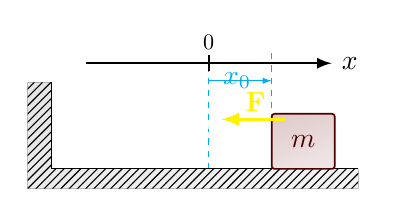
\begin{tikzpicture}
        \def\H{1.1}  % wall height
        \def\T{0.3}  % wall thickness
        \def\W{3.9}  % ground length
        \def\D{0.25} % ground depth
        \def\h{0.7}  % mass height
        \def\w{0.8}  % mass width
        \def\x{2.0}  % mass x position
        \def\dx{0.8} % extension
        \def\y{1.22*\H} % x axis y position
        \def\F{0.8}  % force
        
        % AXIS
        \draw[mydashed] (\x,0) --++ (0,\y) (\x+\dx,0) --++ (0,1.1*\y);
        \draw[axis] (\x-0.4*\W,\y) -- (\x+0.4*\W,\y) node[right] {$x$};
        \tick{\x,\y}{-90} node[scale=0.8,above=-1] {$0$};
        \draw[dx] (\x,1.6*\h) --++ (\dx,0) node[pos=0.45,inner sep=0] {$x_0$};
        
        % SPRING & MASS
        \draw[spring,segment length=7.5] (0,\h/2) --++ (\x+\dx,0);
        \draw[ground] (0,0) |-++ (-\T,\H) |-++ (\T+\W,-\H-\D) -- (\W,0) -- cycle;
        \draw (0,\H) -- (0,0) -- (\W,0);
        \draw[mass] (\x+\dx,0) rectangle++ (\w,\h) node[midway] {$m$};
        \draw[force] (\x+\dx+0.2*\w,0.9*\h) --++ (-\F,0) node[midway,right=1,above=-1] {$\vb{F}$};
        
    \end{tikzpicture}

    Figure 3: Harmonic Oscillator
\end{center}

which gives the time needed to move from $x_0=x(t_0)$ to $x_1=x(t_1)$. To warm up, consider the system of differential equation for the harmonic oscillator, governed by Hooke's law (after normalisation): \[\frac{\D^2}{\D t^2}x(t)=-x(t),\; t\in\R.\]\hfill\T{(harmonic oscillator)}

where $m>0$ is the mass of an object, considered as a point. For $x: \cal{C}^1(\R)$, $t\to x(t)$, define \[E_x:\R\to\R: \quad E_x(t)=\frac12\left(\DD{x}{t}\right)^2+\frac12x^2(t).\]

\tcbcnt{question}{0}
\newq{1e2}{
    Prove that if $x$ satisfies the equation (simple pendulum), then $E_x$ is a constant.
}

\newp{
    Since $E_x$ is continuous and the domain is connected, it suffices to show $E_x'$ is 0, so $\int E_x'(t)\D t = E_x(t)+C$ implies $\int 0\D t = 0 = E_x(t)+C$ and so $E_x(t)=-C$ for some constant $C\in\R$.
    
    To this end, we differentiate $E_x(t)$ with respect to $t$:
    \begin{align*}
        E_x'(t) &= \DD{x(t)}{t}\cd\frac{\D^2 x(t)}{\D t^2} + x(t)\cd\DD{x(t)}{t}\\
        &= \DD{x(t)}{t}\cd(-x(t)) + x(t)\cd\DD{x(t)}{t}\\
        &= (x(t)-x(t))\cd\DD{x(t)}{t}\\
        &= 0.
    \end{align*}

    Hence, we have shown that $E_x$ is a constant.
}

\newq{2e2}{
    Assume that $x$ is a solution of the system with $x_0>0$ being its maximal positive displacement of the object (see the figure). By symmetry, -$x_0$ will be the maximal negative displacement of the object. Prove that if the system starts at $x_0$ (with initial velocity being 0), then \[\D x=-\sqrt{x_0^2-x^2}\D t\] before $x$ passes the origin. From there, compute the minimal period $T$ of $x$, (\ie the minimal time $T$ need for $x$ starting from $x_0$ at $t=0$ and moving back to $x_0$ at time $T$), and show that it is equal to $2\pi$. 

    \newh{
        First find out $\frac{T}{4}$, then use the symmetry of the system.

        \begin{center}
            % PENDULUM + BLOCK
            \def\L{2.6} % length
            \def\ang{-32} % length
            \def\R{0.25} % ball radius
            \def\y{-1.14*\L} % mass
            \begin{tikzpicture}
                \coordinate (M) at (\ang-90:\L);
                \coordinate (M') at (0,-\L);
                \coordinate (O) at (0,0);
                \coordinate (B) at (0,\y);
                \draw[ground] (-0.7*\L,\y) rectangle++ (1.2*\L,-\R);
                \draw (-0.7*\L,\y) --++ (1.2*\L,0);
                \draw[faded mass] (M') circle(\R);
                \draw[dashed] (O) -- (B);
                \rope{(O) -- (M)} \path (O) -- (M) node[midway,left=1] {$L$};
                \fill[black] (O) circle(0.04);
                \draw[mass] (M) circle(\R) node {$m$};
                \draw pic["$x_0$",angle radius=15,angle eccentricity=1.3] {angle=M--O--B};
            \end{tikzpicture}

            Figure 4: Simple pendulum
        \end{center}

        Now consider the system of differential equation for the simple pendulum, governed by gravity (after normalisation): \[\frac{\D^2}{\D t^2}x(t)=-\sin(x(t)),\; t\in\R.\]\hfill\T{(simple pendulum)} 
        
        where $m>0$ is the mass of an object, considerd as a point, $x$ is the (signed) angle formed by the rod and the vertical line. For simplicity, let's assume by convention that when the rod is to the left of the vertical dash line, we say the angle is positive, when the rod is to the right of the vertical dash line, we say the angle is negative.

        For $x:\cal{C}^1(\R)$, $t\to x(t)$, define \[E_x:\R\to\R: \quad E_x(t)=\frac12\left(\DD{x}{t}\right)^2+(1-\cos(x(t))).\]
    }
}

\newp{
    Using the equation from Exercise 2 Question \ref{question:q1e2}, we have $E_x(t)=\frac12\left(\DD{x}{t}\right)^2+\frac12(x^2(t))$ which is a constant. Since $\DD{x(t)}{t}=0$ at $t=0$ and $x(0)=x_0$, we have \begin{align*}
        E_{x_0}(t) &= E_x(t)\\
        \frac12 (0)^2 + \frac12 x_0^2 (t) &= \frac12 \bra{\DD{x}{t}}^2 + \frac12 x^2(t)\\
        \DD{x}{t} &= \pm\sqrt{x_0^2-x^2}.\\
        \alt{To show $T=2\pi$, it suffices to show the time from $x_0$ to $0$ is fourth of the period by symmetry. To this end, we will show $\int_{x_0}^0\D t = \frac{\pi}{2}$. Since from $x_0$ to $0$, the velocity $\DD{x}{t}$ is always non-positive (decreasing), we have}
        \DD{x}{t} &= -\sqrt{x_0^2-x^2}\\
        \D t &= -\frac{\D x}{\sqrt{x_0^2-x^2}}\\
        \int_{x_0}^0 \D t &= -\int_{x_0}^0 \frac{\D x}{\sqrt{x_0^2-x^2}}\\
        &= \int_0^{x_0} \frac{\D x}{\sqrt{x_0^2-x^2}}\\
        \alt{Since $\int\frac{1}{\sqrt{a^2-x^2}}\D x=\arcsin\frac{x}{a}+C$, we have}
        &= \arcsin\frac{x}{x_0}\Big|_0^{x_0}\\
        &= \arcsin\frac{x_0}{x_0}-\arcsin\frac{0}{x_0}\\
        &= \arcsin 1 - \arcsin 0\\
        &= \frac{\pi}{2} - 0\\
        &= \frac{\pi}{2}.
    \end{align*}

    Hence, we have shown that $\frac{T}{4}=\frac{\pi}{2}$, by symmetry this implies $T=2\pi$, which completes our proof. 
}

\newq{3e2}{
    Prove that if $x$ satisfies the equation (simple pendulum), then $E_x$ is a constant.
}

\newp{
    Similar to Exercise 2 Question \ref{question:q1e2}, we will show that $E_x$ is a constant by showing that $E_x'=0$. To this end, we differentiate $E_x(t)$ with respect to $t$:
    \begin{align*}
        E_x'(t) &= \DD{x(t)}{t}\cd\frac{\D^2 x(t)}{\D t^2} + \sin(x(t))\cd\DD{x(t)}{t}\\
        &= \DD{x(t)}{t}\cd(-\sin(x(t))) + \sin(x(t))\\
        &= 0.
    \end{align*}

    Hence, we have shown that $E_x$ is a constant since $E_x'\is0$  .
}

\newq{4e2}{
    Assume that $x$ is a solution of the system with $x_0>0$ being its maximal positive angle (see the figure). By symmetry, $-x_0$ will be the maximal negative angle of the object. Prove that if the system starts at $x_0$ (with initial velocity being 0), then \[\D x=-\sqrt{2(\cos x-\cos x_0)}\D t\] before the rod becomes vertical (\ie when $x$ reaches 0). From there, compute the minimal period $T$ of $x$, (\ie the minimal time $T$ need for $x$ starting from $x_0$ at $t=0$ and moving back to $x_0$ at time $T$), show that it is an elliptic integral of the first type.
}

\newp{
    Using the formula \[E_x(t)=\frac12\bra{\DD{x}{t}}^2+(1-\cos(x(t))),\] and at $x_0$, we can see $\DD{x_0}{t}$ is 0, and \begin{align*}
        \frac12\bra{\DD{x}{t}}^2+(1-\cos(x(t))) &= \frac12\bra{0}^2+(1-\cos(x_0))\\
        \DD{x}{t} &= \pm\sqrt{2(\cos x-\cos x_0)}.
        \alt{Since the velocity is non-positive from $x_0$ to $0$, we have}
        \D x &= -\sqrt{2(\cos x-\cos x_0)}\D t\\
        \D t &= -\frac{\D x}{\sqrt{2(\cos x-\cos x_0)}}\\
        &=-\frac{1}{\sqrt2}\cd\frac{\D x}{\sqrt{\cos x - \cos x_0}}\\
        4\cd\int_{x_0}^0 \D t&=-\frac{4}{\sqrt2}\int_{x_0}^0 \frac{\D x}{\sqrt{\cos x - \cos x_0}}\\
        T &= - 2\sqrt2\int_{x_0}^0 \frac{\D x}{\sqrt{\cos x - \cos x_0}}.
        \alt{Now, it suffices to show the integral $\int_{x_0}^0 \frac{\D x}{\sqrt{\cos x - \cos x_0}}$ is in the form of $E_1$, thus we cannot find finitely many elementary functions to represent it. So,}
        \int_{x_0}^0\frac{\D x}{\sqrt{\cos x - \cos x_0}} &= \int_{x_0}^0\frac{\D x}{\sqrt{1 - \sin^2\bra{\frac{ x}{2}} - 1 + \sin^2 \bra{\frac{x_0}{2}}}}\\
        &=\int_{x_0}^0\frac{\D x}{\sqrt{\sin^2\bra{\frac{x_0}{2}}-\sin^2\bra{\frac{x}{2}}}}\\
        &=\int_{x_0}^0\frac{\frac{1}{\sin \bra{\frac{x_0}{2}}}\D x}{\sqrt{1-\frac{1}{\sin^2\bra{\frac{x_0}{2}}}\cd\sin^2\bra{\frac{x}{2}}}}\\
        \alt{Let $\sin\th=\frac{\sin\bra{\frac{x}{2}}}{\sin\bra{\frac{x_0}{2}}}$, then $\cos\bra{\frac{x}{2}}\frac{\D x}{2}=\cos\th\sin\bra{\frac{x_0}{2}}\D \th$ which gives}
        \D x &= \frac{2\sin\bra{\frac{x_0}{2}}\cos\th\D \th}{\cos\bra{\frac{x}{2}}}\\
        \cos\th&=\sqrt{1-\sin^2\th}=\sqrt{1-\frac{\sin^2\bra{\frac{x}{2}}}{\sin^2\bra{\frac{x_0}{2}}}}\\
        \cos\bra{\frac{x}{2}}&=\sqrt{1-\sin^2\bra{\frac{x}{2}}}\\
        \D x &= \frac{2\sin\bra{\frac{x_0}{2}}\sqrt{1-\frac{\sin^2\bra{\frac{x}{2}}}{\sin^2\bra{\frac{x_0}{2}}}}}{\sqrt{1-\sin^2\bra{\frac{x}{2}}}}\D \th\\
        &=\frac{2\sqrt{\sin^2\bra{\frac{x_0}{2}}-\sin^2\bra{\frac{x}{2}}}}{\sqrt{1-\sin^2\bra{\frac{x_0}{2}}\cd\sin^2\th}}\D \th
        \alt{Substitute into our integral, $x_0\in(0, \pi)$ and $x\in(0,x_0)$ implies $\sin\th\in(\frac{\sin(0)}{\sin(\frac{x_0}{2})},\frac{\sin(\frac{x_0}{2})}{\sin(\frac{x_0}{2})})=(0, 1)$, so $\th\in(0,\frac{\pi}{2})$ and we have}
        \int_{x_0}^0\frac{\frac{1}{\sin \bra{\frac{x_0}{2}}}\D x}{\sqrt{\cos x - \cos x_0}} &=2\int_{\frac{\pi}{2}}^0\frac{1}{\sqrt{1-\frac{1}{\sin^2\bra{\frac{x_0}{2}}}\cd\sin^2\bra{\frac{x}{2}}}}\cd\frac{2\sqrt{\sin^2\bra{\frac{x_0}{2}}-\sin^2\bra{\frac{x}{2}}}}{\sqrt{1-\sin^2\bra{\frac{x_0}{2}}\cd\sin^2\th}}\cd\frac{1}{\sin \bra{\frac{x_0}{2}}}\D \th\\
        &=4\int_{\frac{\pi}{2}}^0\frac{\sqrt{\sin^2\bra{\frac{x_0}{2}}-\sin^2\bra{\frac{x}{2}}}}{\sqrt{(1-\frac{1}{\sin^2\bra{\frac{x_0}{2}}}\cd\sin^2\bra{\frac{x}{2}})\cd(1-\sin^2\bra{\frac{x_0}{2}}\cd\sin^2\th)}}\cd\frac{1}{\sin \bra{\frac{x_0}{2}}}\D \th\\
        &=4\int_{\frac{\pi}{2}}^0\frac{\sqrt{\sin^2\bra{\frac{x_0}{2}}-\sin^2\bra{\frac{x}{2}}}}{\sqrt{1-\frac{1}{\sin^2\bra{\frac{x_0}{2}}}\cd\sin^2\bra{\frac{x}{2}}-\sin^2\bra{\frac{x_0}{2}}\cd\sin^2\th+\sin^2\bra{\frac{x}{2}}\sin^2\th}}\cd\frac{1}{\sin \bra{\frac{x_0}{2}}}\D \th\\
        &=4\int_{\frac{\pi}{2}}^0\frac{1}{\sqrt{\frac{1-\frac{1}{\sin^2\bra{\frac{x_0}{2}}}\cd\sin^2\bra{\frac{x}{2}}-\sin^2\bra{\frac{x_0}{2}}\cd\sin^2\th+\sin^2\bra{\frac{x}{2}}\sin^2\th}{\sin^2\bra{\frac{x_0}{2}}-\sin^2\bra{\frac{x}{2}}}}}\cd\frac{1}{\sin \bra{\frac{x_0}{2}}}\D \th\\
        &=4\int_{\frac{\pi}{2}}^0\frac{1}{\sqrt{
            \frac{
                1-\frac{1}{\sin^2\bra{\frac{x_0}{2}}}\cd\sin^2\bra{\frac{x}{2}}
            }{
                \sin^2\bra{\frac{x_0}{2}}-\sin^2\bra{\frac{x}{2}}
            }
            +\frac{
                -\sin^2\bra{\frac{x_0}{2}}\cd\sin^2\th+\sin^2\bra{\frac{x}{2}}\sin^2\th
            }{
                \sin^2\bra{\frac{x_0}{2}}-\sin^2\bra{\frac{x}{2}}
            }
        }}\cd\frac{1}{\sin \bra{\frac{x_0}{2}}}\D \th\\
        &=4\int_{\frac{\pi}{2}}^0\frac{1}{\sqrt{
            \frac{
                1-\frac{1}{\sin^2\bra{\frac{x_0}{2}}}\cd\sin^2\bra{\frac{x}{2}}
            }{
                \sin^2\bra{\frac{x_0}{2}}-\sin^2\bra{\frac{x}{2}}
            }
            -\sin^2\th
        }}\cd\frac{1}{\sin \bra{\frac{x_0}{2}}}\D \th\\
        &=4\int_{\frac{\pi}{2}}^0\frac{1}{\sqrt{
            \frac{
                1-\sin^2\th
            }{
                \sin^2\bra{\frac{x_0}{2}}-\sin^2\bra{\frac{x}{2}}
            }
            -\sin^2\th
        }}\cd\frac{1}{\sin \bra{\frac{x_0}{2}}}\D \th\\
        &=4\int_{\frac{\pi}{2}}^0\frac{1}{\sqrt{
            \frac{1}{\sin^2\bra{\frac{x_0}{2}}}\frac{
                1-\sin^2\th
            }{
                1-\sin^2\th
            }
            -\sin^2\th
        }}\cd\frac{1}{\sin \bra{\frac{x_0}{2}}}\D \th\\
        &=4\int_{\frac{\pi}{2}}^0\frac{1}{\sqrt{
            \frac{1}{\sin^2\bra{\frac{x_0}{2}}}
            -\sin^2\th
        }}\cd\frac{1}{\sin \bra{\frac{x_0}{2}}}\D \th\\
        &=4\int_{\frac{\pi}{2}}^0\frac{\sin\bra{\frac{x_0}{2}}}{\sqrt{
            1
            -\sin^2\bra{\frac{x_0}{2}}\sin^2\th
        }}\cd\frac{1}{\sin \bra{\frac{x_0}{2}}}\D \th\\
        &=4\int_{\frac{\pi}{2}}^0\frac{\sin\bra{\frac{x_0}{2}}}{\sqrt{
            1
            -\sin^2\bra{\frac{x_0}{2}}\sin^2\th
        }}\cd\frac{1}{\sin \bra{\frac{x_0}{2}}}\D \th\\
        &=4\int_{\frac{\pi}{2}}^0\frac{1}{\sqrt{
            1
            -\sin^2\bra{\frac{x_0}{2}}\sin^2\th
        }}\D \th\\
        \alt{Let $k=\sin\bra{\frac{x_0}{2}}$, then from the domain of $x_0$ we have $k\in(0,1)$ (can never reach the end points), and}
        &=4\int_{\frac{\pi}{2}}^0\frac{1}{\sqrt{
            1-k^2\sin^2\th
        }}\D \th\\
        \alt{Which is indeed the elliptic integral of the first kind, $E_1=\int\frac{1}{\sqrt{1-k^2\sin^2\th}}\D \th$.}
    \end{align*}

    Therefore, we conclude $T=-2\sqrt{2}\cd\bra{4\int_{\frac{\pi}{2}}^0\frac{1}{\sqrt{1-k^2\sin^2\th}}\D \th}=8\sqrt{2}\int_{0}^{\frac{\pi}{2}}\frac{1}{\sqrt{1-k^2\sin^2\th}}\D \th$ is the minimal period of arbitrary $x_0$, and is an elliptic integral of the first kind as shown.
}

From now on, consider the period $T=T(x_0)$ as a function of $x_0$.

\newq{5e2}{
    Prove that \[\lim_{x_0\to 0} T(x_0)=2\pi.\]
}

\newp{
    We will use the Taylor Expansion of $\cos$ at $x=0$, that is, the Maclaurin Expansion of $\cos$: $\cos x = 1 - \frac{x^2}{2} + \cdots$.

    When $x_0\to 0$, we have \begin{align*}
        T&=-\frac{4}{\sqrt2}\int_{x_0}^0\frac{\D x}{\sqrt{\cos x - \cos x_0}}\\
        &\approx\frac{4}{\sqrt2}\int_{0}^{x_0}\frac{\sqrt2 \D x}{\sqrt{x_0^2-x^2}}\\
        &=4\int_{0}^{x_0}\frac{\D x}{\sqrt{x_0^2-x^2}}\\
        \alt{Let $x=x_0\sin\th$, then $\sqrt{x_0^2-x^2}=x_0\cos\th$, and $\D x=x_0\cos\th\D \th$, so $x\in(0,x_0)$ implies $\th\in(0,\frac{\pi}{2})$, and}
        &=4\int_{0}^{\frac{\pi}{2}}\frac{x_0\cos\th\D \th}{x_0\cos\th}\\
        &=4\int_{0}^{\frac{\pi}{2}}\D \th\\
        &=4\bra{\th}\Big|_0^{\frac{\pi}{2}}\\
        &=2\pi.
    \end{align*}
}

\newq{6e2}{
    Prove that \[\lim_{x_0\to\pi} T(x_0)=\infty.\]
}

\newp{
    Since $T=\frac{4}{\sqrt2}\int_0^{x_0}\frac{\D x}{\sqrt{\cos x - \cos x_0}}$, when $x_0\to\pi$, to show $\lim_{x_0\to\pi} T(x_0)=\infty$, it suffices to show that the integral $\int_0^{\pi}\frac{\D x}{\sqrt{\cos x - \cos \pi}}=\int_0^{\pi}\frac{\D x}{\sqrt{\cos x + 1}}$ diverges to infinity.

    To this end, we show $\frac{1}{\sqrt{\cos x + 1}}$ is unbounded as $x\to\pi$. So, clearly $\lim_{x\to\pi}\frac{1}{\sqrt{\cos x + 1}}=\infty$, and so $\lim_{x_0\to\pi} T(x_0)=\infty$.
}

\newr{
    These two exercises demonstrate that although the Newton-Leibniz formula is a powerful tool in computing the definite integrals, many (nonlinear) problems raising from geometry and physics can \tbf{not} be explicitely computed. Rather, the integral itself is an important approach to \tbf{construct} new functions (for exmaple the elliptic functions, which are the inverses of elliptic integrals).
}

\end{document}